\subsection{The Challenges: Foregrounds, systematics}
\label{sec:foregrounds}
\vspace{-0.05in}
\comred{3 pages. Discuss the challenge of Foregrounds and Systematics. }
%A satellite mission provides a unique opportunity to target both the inflationary B-mode polarization that originates from the epoch of recombination and peaks around $\ell=80$ and the contribution that peaks on significantly larger scales $\ell\lesssim 12$. To measure the contribution from reionization will require an unprecedented understanding of foregrounds and systematic effects. This is illustrated in the left panel of Figure~\ref{fig:Qrp001}, which shows the contribution from reionization to the Stokes $Q$-parameter for $r=0.001$. The amplitude of the signal is approximately $10$ nK

A satellite mission provides the best  both the inflationary B-mode polarization that originates from the epoch of recombination and peaks around $\ell=80$ and the contribution from reionization that peaks on significantly larger scales at $\ell\lesssim 12$. The contribution from reionization to the Stokes $Q$-parameter for a tensor-to-scalar ratio $r=0.001$ in the left panel of Figure~\ref{fig:Qrp001}. The amplitude of the signal is approximately $10$ nK so that both residual foregrounds and systematics must be controlled at an unprecedented level of a few nK.

\begin{figure}[h]
\begin{center}
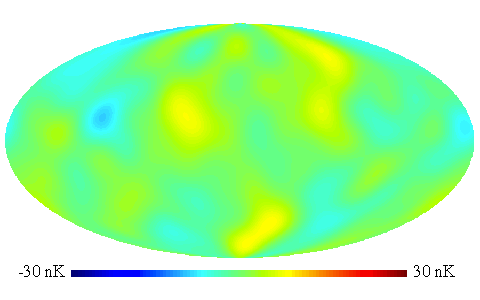
\includegraphics[width=3.2in]{Figures/P15_2_12_rp001.pdf}
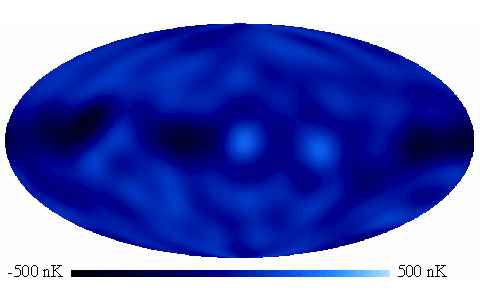
\includegraphics[width=3.2in]{Figures/P353_N_2_12.pdf}
\end{center}
\caption{{\it Left panel:} Contribution to the Stokes $Q$ parameter from inflationary B-modes for $\ell<12$ for $r=0.001$. {\it Right panel:} Noise in the $Planck$ 353 GHz map of the Stokes $Q$ parameter for $\ell<12$ rescaled to 150 GHz assuming the spectral properties of dust.}
\label{fig:Qrp001}
\end{figure}

Data from the $Planck$ satellite has recently led to a significant improvement in our understanding of foregrounds in both intensity and polarization. In intensity, $Planck$, for example, showed the unexpected relevance of Carbon-Monoxide lines at moderate latitudes as well as the existence of an anomalous emission from dust at low frequencies. In polarization, the sky appears to be dominated by the expected polarized foregrounds, synchrotron and dust. Our knowledge is limited, of course, by the sensitivity of Planck, and this does not mean that additional components, especially anomalous dust, could not have a certain degree of polarization. 

$Planck$ has also provided us with much improved measurements of the amplitude and spectral dependence of synchrotron emission and dust. The spectral dependence of both foregrounds and signal is summarized in the left panel of Figure~\ref{fig:frequency} for different sky fractions. The power spectrum of foregrounds over $75\%$ of the sky for frequencies between $70$ and $200$ GHz is shown in the right panel, together with the inflationary contribution for different values of the tensor-to-scalar ratio.

\begin{figure}[h]
\begin{center}
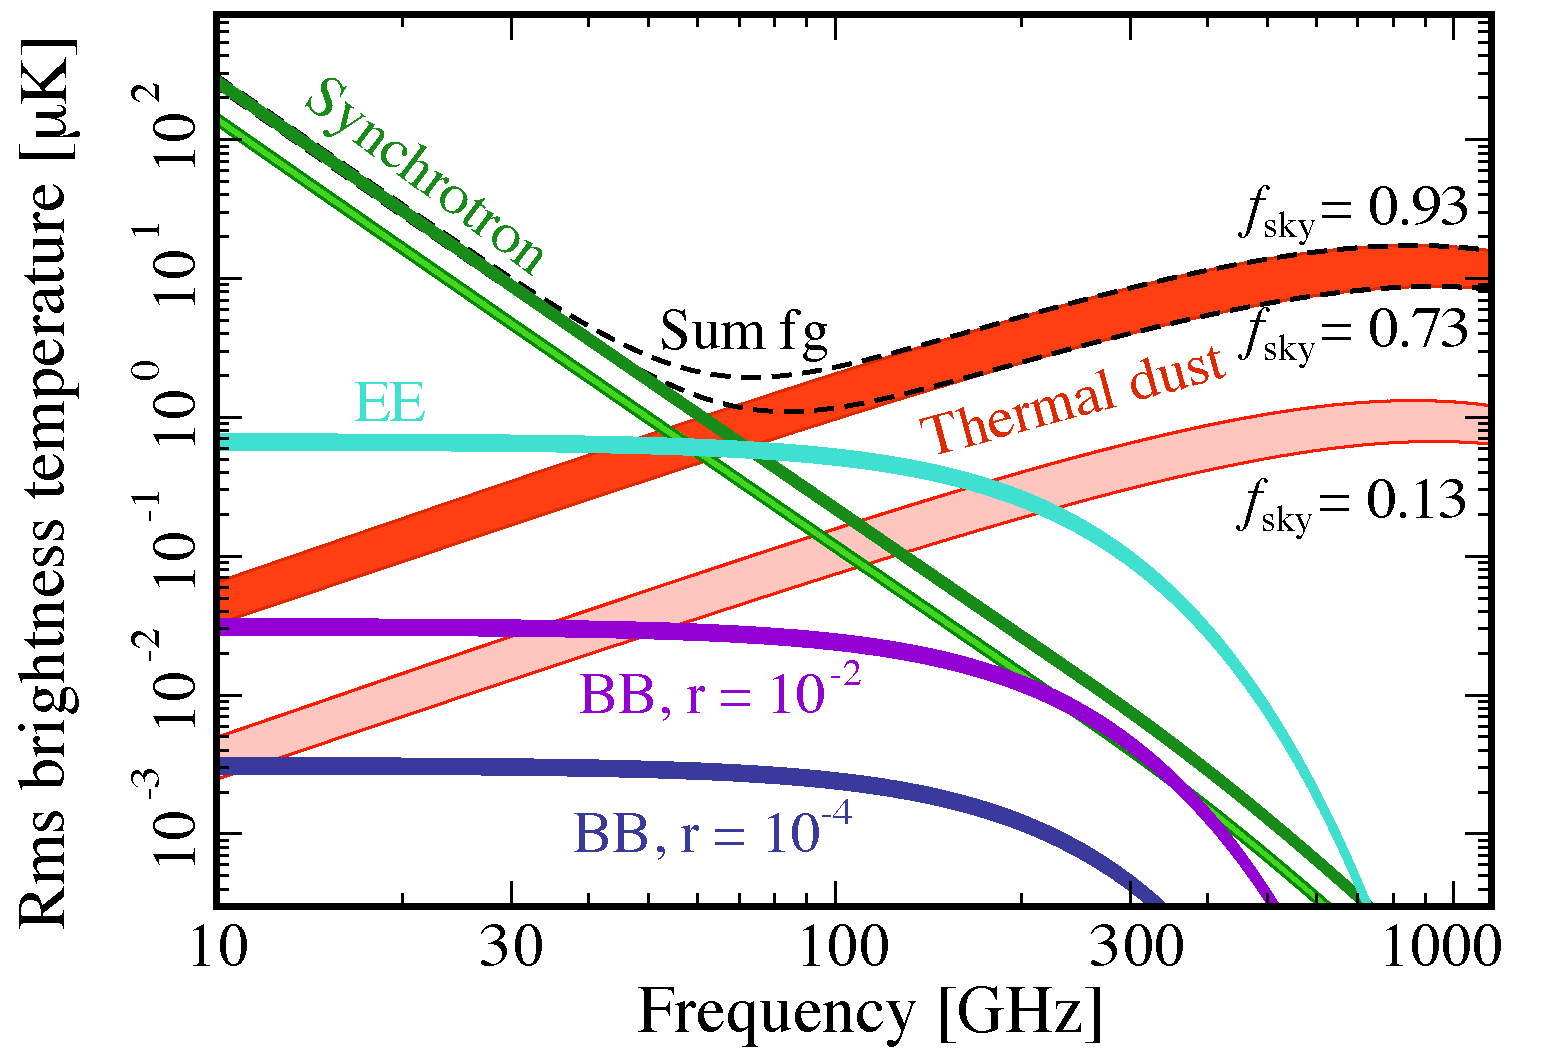
\includegraphics[width=3.26in]{Figures/overview_pol_v4_fsky_noplanck.pdf}\hskip .2cm
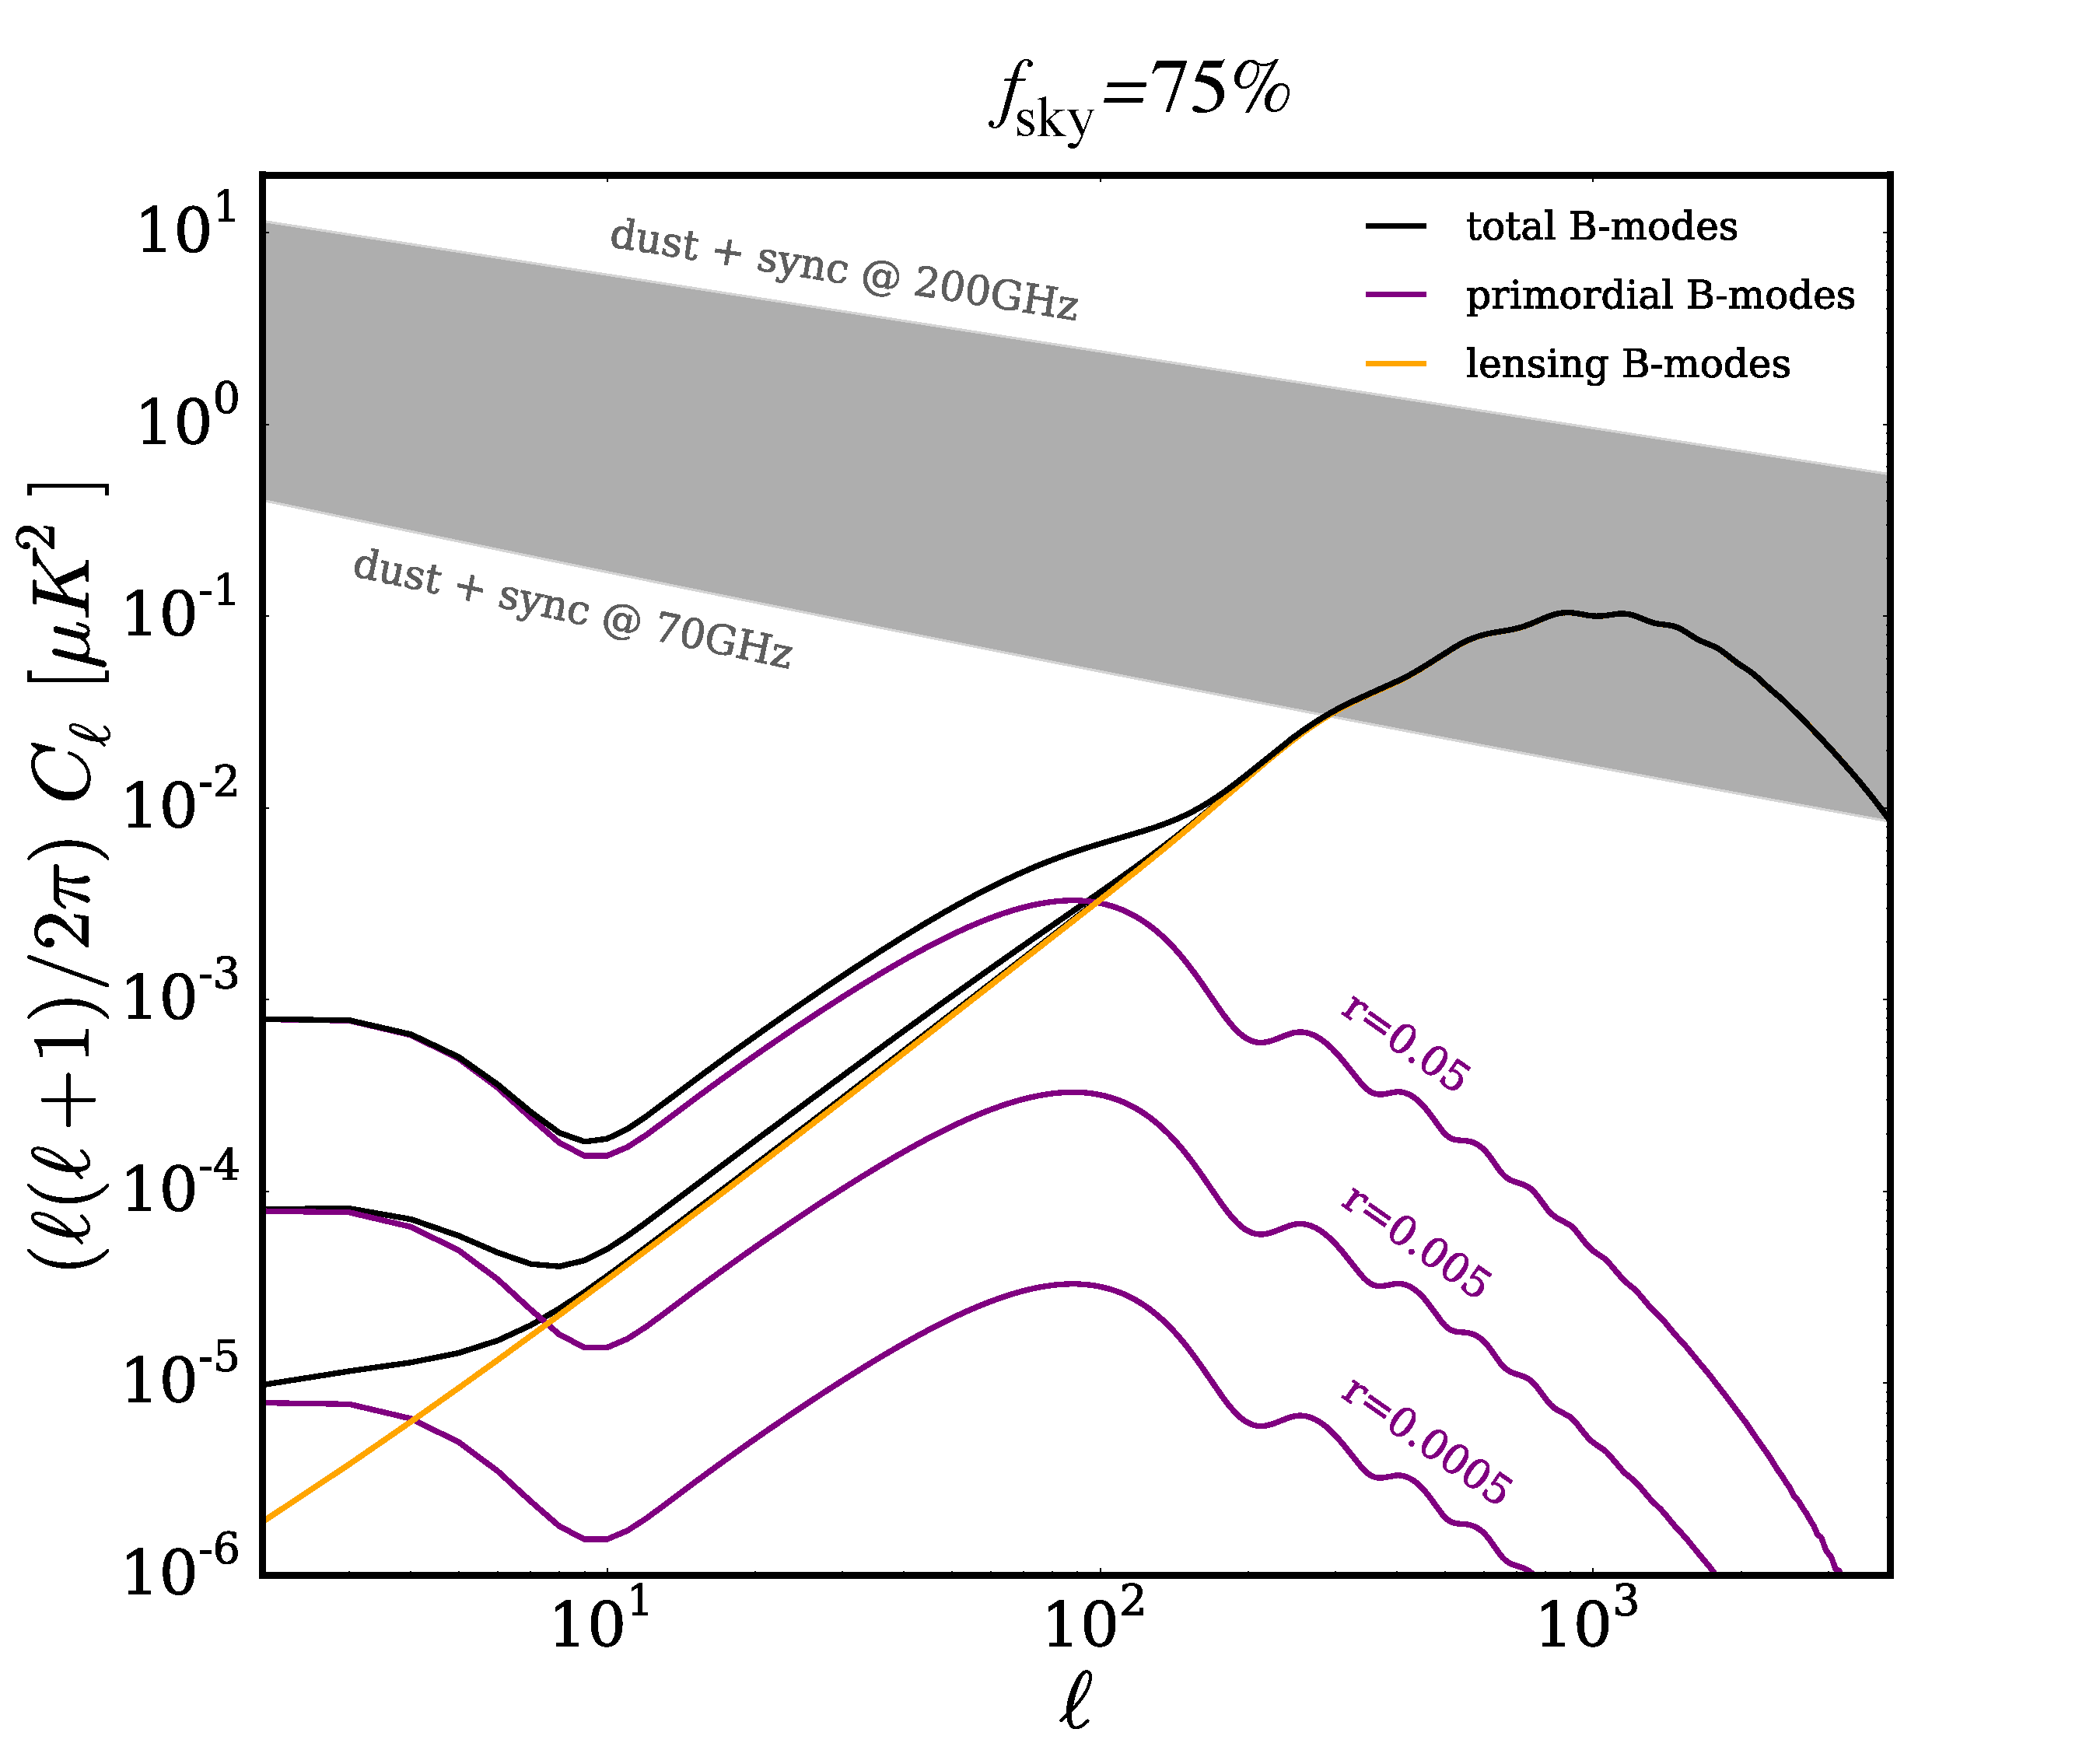
\includegraphics[width=3.12in]{Figures/clbb_freq.pdf}
\end{center}
\caption{{\it Left panel:} Brightness temperature as function of frequency for the CMB as well as synchrotron emission (green) and dust emission (red). The darker bands show the brightness temperature for sky fractions between $73\%$ and $93\%$, the lighter bands show the brightness temperature for the cleanest $13\%$ with the width indicating the uncertainty. {\it Right panel:} Angular power spectrum for B-mode polarization of the CMB for $r=0.0005$, $r=0.005$, and $r=0.05$ as well as for foreground emission between 70 and 200 GHz.}
\label{fig:frequency}
\end{figure}

Perfect knowledge of the foreground components would allow to remove them, but the sensitivity of Planck sets limits. The right panel in Figure~\ref{fig:Qrp001} shows the noise in the $Planck$ map of the Stokes $Q$-parameter at 353 GHz rescaled to 150 GHz assuming the same spectral dependence as for dust and on the angular scales relevant for the measurement of the inflationary $B$-modes on large angular scales. The noise is more than an order of magnitude larger than the inflationary contribution for $r=0.001$, clearly indicating the necessity to measure foregrounds with a potential future space mission. 

One of the key ingredients in the design of a CMB experiment is the frequency coverage required to achieve the science goals. Consequently, optimizing frequency coverage in light of the new information from $Planck$ and its limitations will be one of key task of the study proposed here.   

% Raphael, Josquin, Aurelien, Charles
